%----------------------------------------------------------------------------------------
%	PACKAGES AND OTHER DOCUMENT CONFIGURATIONS
%----------------------------------------------------------------------------------------

\documentclass[
12pt,
a4paper,
onecolumn,
portrait
]{article}

%%%%%%%%%%%%%%%%%%%%%%%%%%%%%%%%%%%%%%%%%
% Article Notes
% Structure Specification File
% Version 1.0 (1/10/15)
%
% This file has been downloaded from:
% http://www.LaTeXTemplates.com
%
% Authors:
% Vel (vel@latextemplates.com)
% Christopher Eliot (christopher.eliot@hofstra.edu)
% Anthony Dardis (anthony.dardis@hofstra.edu)
%
% License:
% CC BY-NC-SA 3.0 (http://creativecommons.org/licenses/by-nc-sa/3.0/)
%
%%%%%%%%%%%%%%%%%%%%%%%%%%%%%%%%%%%%%%%%%

%----------------------------------------------------------------------------------------
%	REQUIRED PACKAGES
%----------------------------------------------------------------------------------------

\usepackage[includeheadfoot,columnsep=2cm, left=1in, right=1in, top=.5in, bottom=.5in]{geometry} % Margins

%\usepackage[T1]{fontenc} % For international characters
\usepackage[utf8]{inputenc}
%\usepackage{XCharter} % XCharter as the main font

\usepackage{natbib} % Use natbib to manage the reference
%\usepackage{cite}
%\bibliographystyle{apalike} % Citation style
%\bibliographystyle{te} % Citation style

\usepackage[english]{babel} % Use english by default
\usepackage{amsmath}
\usepackage{amssymb}
\usepackage{amsthm}
\usepackage{xcolor}
\usepackage{graphicx}
\usepackage{enumerate}
\usepackage{todonotes}

\newtheorem{df}{Definition}
\newtheorem{ex}{Example}
\newtheorem{as}{Assumption}
\newtheorem{rem}{Remark}
\newtheorem{pr}{Proposition}
\newtheorem{qu}{Question}
\newtheorem{lm}{Lemma}

%----------------------------------------------------------------------------------------
%	CUSTOM COMMANDS
%----------------------------------------------------------------------------------------

\newcommand{\articletitle}[1]{\renewcommand{\articletitle}{#1}} % Define a command for storing the article title
%\newcommand{\articlecitation}[1]{\renewcommand{\articlecitation}{#1}} % Define a command for storing the article citation
\newcommand{\doctitle}{``\articletitle''} % Define a command to store the article information as it will appear in the title and header

\newcommand{\datenotesstarted}[1]{\renewcommand{\datenotesstarted}{#1}} % Define a command to store the date when notes were first made
\newcommand{\docdate}[1]{\renewcommand{\docdate}{#1}} % Define a command to store the date line in the title

\newcommand{\docauthor}[1]{\renewcommand{\docauthor}{#1}} % Define a command for storing the article notes author

% Define a command for the structure of the document title
\newcommand{\printtitle}{
\begin{center}
\textbf{\Large{\doctitle}}

\docdate

\docauthor
\end{center}
}

% set interior
\newcommand{\interior}[1]{%
  {\kern0pt#1}^{\mathrm{o}}%
}

%----------------------------------------------------------------------------------------
%	STRUCTURE MODIFICATIONS
%----------------------------------------------------------------------------------------

\setlength{\parskip}{3pt} % Slightly increase spacing between paragraphs

% Uncomment to center section titles
%\usepackage{sectsty}
%\sectionfont{\centering}

% Uncomment for Roman numerals for section numbers
%\renewcommand\thesection{\Roman{section}}


%----------------------------------------------------------------------------------------
%	ARTICLE INFORMATION
%----------------------------------------------------------------------------------------

\articletitle{Notes on our common PDE model} % The title of the article
\datenotesstarted{October 17, 2016} % The date when these notes were first made
\docdate{\datenotesstarted; rev. \today} % The date when the notes were lasted updated (automatically the current date)

\docauthor{Julian Andrej, Luca Mechelli, \underline{Simon Pirkelmann}} % Your name

%----------------------------------------------------------------------------------------

\begin{document}

\pagestyle{myheadings} % Use custom headers
\markright{\doctitle} % Place the article information into the header

%----------------------------------------------------------------------------------------
%	PRINT ARTICLE INFORMATION
%----------------------------------------------------------------------------------------

\thispagestyle{plain} % Plain formatting on the first page

\printtitle % Print the title

%----------------------------------------------------------------------------------------
%	ARTICLE NOTES
%----------------------------------------------------------------------------------------
\section{Model}
\subsection{Model equations}
I propose we use the following simulation model:
\begin{align}
\frac{\partial \mathbf{y_1}}{\partial t} + \mathbf{y_1} \cdot \nabla \mathbf{y_1} &= - \frac{1}{\rho} \nabla y_2 + \nu \Delta \mathbf{y_1} - \textbf{g} \alpha \Delta y_3 \label{eq:pde-navier-stokes}\\
\nabla \cdot \mathbf{y_1} &= 0 \label{eq:pde-continuity}\\
\frac{\partial y_3}{\partial t} + \mathbf{y_1} \cdot \nabla y_3 &= \kappa \Delta y_3 \label{eq:pde-heat-equation}
\end{align}
\begin{align*}
& \mathbf{y_1}: \Omega \times [0, \infty) \rightarrow \mathbb{R}^{d} \text{ is air velocity}  \\
\text{where}\;\;\; &y_2: \Omega \times [0, \infty) \rightarrow \mathbb{R} \;\; \text{ is pressure} \\
&y_3: \Omega \times [0, \infty) \rightarrow \mathbb{R} \;\; \text{ is temperature}
\end{align*}
and coefficients 
\begin{align*}
\rho &: \text{ density of the fluid } \\
\nu  &: \text{ kinematic viscosity } \\
\alpha &: \text{ coefficient of expansion } \\
\kappa &: \text{ thermal diffusivity. } \\
\end{align*}
Some explanation: This model is the so-called Boussinesq approximation of the Navier-Stokes equations, which makes the simplifying assumption that the density of the fluid is constant, which leads to equation \eqref{eq:pde-continuity} (instead of $\frac{\partial \rho}{\partial t} + \nabla \cdot (\rho \mathbf{y_1}) = 0$ in the general form). Equation \eqref{eq:pde-navier-stokes} is the Boussinesq dynamical equation for describing the air flow and equation \eqref{eq:pde-heat-equation} is the equation for the temperature transfer (convection-diffusion). Here the assumption is made that no heat is generated within the domain, i.e. there is no reaction (or source) term.\\
Note that the states $\mathbf{y_1}$ and $y_3$ are directly coupled. This is clear from a physical point of view. A change in temperature ($\Delta y_3$) causes the air to expand or contract which in turn induces an air flow and thus influences the state $\mathbf{y_1}$ (equation \eqref{eq:pde-navier-stokes}). On the other hand the air velocity determines the direction in which the convection term $\nabla y_3$ acts on the temperature in equation \eqref{eq:pde-heat-equation}.

\subsection{Boundary conditions}
Consider the following boundary conditions to the problem
\begin{align}
\mathbf{y_1} &= 0 &\text{ on } &\Gamma \times [0, \infty) \label{eq:pde-boundary-air-velocity-dirichlet} \\
\partial_{\nu} y_3 &= u + f &\text{ on } &\Gamma_1  \times [0, \infty) \label{eq:pde-boundary-heating}\\
\partial_{\nu} y_3 &= f &\text{ on } &(\Gamma \setminus \Gamma_1)  \times [0, \infty) \label{eq:pde-boundary-no-heating}
\end{align}
where $u: \Gamma_1 \times [0, \infty) \rightarrow \mathbb{R}$, $f: \Gamma \times [0, \infty) \rightarrow \mathbb{R}$. \\
The motivation for using these boundary conditions is as follows. The function $f$ can be considered as an outside temperature that influences the temperature within the domain via the boundary. The boundary is split up in two parts. On the boundary segment $\Gamma_1$ we can control the heating by the function $u$ specifying the heat flux across the boundary, which also allows us to influence the temperature $y_3$ (equation \eqref{eq:pde-boundary-heating}). The other part of the boundary ($\Gamma \setminus \Gamma_1$) is not heated (equation \eqref{eq:pde-boundary-no-heating}). \\
We also impose a Dirichlet boundary condition for the air velocity $\mathbf{y_1}$ (equation \eqref{eq:pde-boundary-air-velocity-dirichlet}). This expresses that (for now) we assume that there is no air flow into or out of the domain. \\
Note that we do not impose boundary conditions on the pressure $y_2$. Instead the pressure should be determined naturally through the model equations.

\subsection{Domain}
For now let's start in 2D and consider the following simple domain:
\begin{align*}
\Omega &= [0, 1] \times [0, 1] \subset \mathbb{R}^{2} \\
\Gamma &= \Omega \setminus \interior{\Omega} \\
\Gamma_1 &= [0, 1] \times \{0\}
\end{align*}
\begin{figure}[h]
\centering
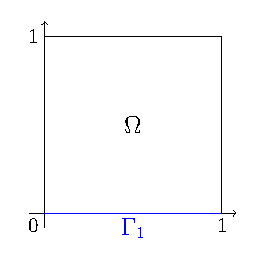
\includegraphics[scale=1.5]{../graphics/domain.pdf}
\caption{Illustration of the domain and the boundary.}
\label{fig:domain-simple}
\end{figure}

\begin{rem}
Some general remarks and questions regarding the model
\begin{enumerate}
\item Coming from the direction of optimal control I prefer the notation $\mathbf{y_i}$ for the state and $u$ for the control. However, this notation does not directly convey the physical interpretation of the state in the model. We can adapt this if you want, i.e. use e.g. $\mathbf{v}$, $p$ and $T$ for the states. What do you think?
\item 
Julian mentioned that from a numerics point of view it would be preferable to change equation \eqref{eq:pde-continuity} to
\begin{equation}
\nabla \cdot \mathbf{y_1} = \varepsilon y_2
\end{equation}
with a small $\varepsilon > 0$ to have a more direct coupling between pressure and air velocity. I chose not to include it in the model equations above, but I wanted to mentioned it here.
\item Should we consider other types of boundary conditions right away? Right now we only have one control (the heating) but no ventilation. Adding this would lead to a different boundary condition of Neumann-type for the state $\mathbf{y_1}$.
\item What kind of 2D are we looking at? We could interpret the domain as a cut-through of a three-dimensional room, but we should specify if we consider it top-down or as a side-view.\\
Julian and I talked about this briefly and both of us naturally preferred (or rather intuitively thought of) the top-down way. However, I then have difficulty understanding how the gravity acts on the system.  On the right hand side of the Navier-Stokes equation \eqref{eq:pde-navier-stokes} there appears the term $- \textbf{g} \alpha \Delta y_3$. In this expression there appears the vector $\mathbf{g}$. I think in the top-down setting the temperature does not have any influence on the air velocity, because this gravity vector just disappears. I may be wrong about this; if so please help me understand this better. Otherwise we should maybe focus on the side-view approach.
\item How to choose parameters/coefficients? Since I do not have too much experience with the physics I didn't specify the values. Does it make sense to use just constant values of $1$? I guess we can also just use values from the literature, but I haven't looked for the appropriate parameters for air yet.
\end{enumerate}
\end{rem}


\section{Weak form}
TODO!

%----------------------------------------------------------------------------------------
%	BIBLIOGRAPHY
%----------------------------------------------------------------------------------------
\newpage
\renewcommand{\refname}{Reference} % Change the default bibliography title

\nocite{tritton2012physical}

\bibliography{../bibtex} % Input your bibliography file
\bibliographystyle{plain}


%----------------------------------------------------------------------------------------

\end{document}
